\section{Stand der Forschung}

In diesem Kapitel wird der aktuelle Stand der Forschung im Kontext dieser Arbeit dargestellt. Der Fokus liegt dabei auf bestehenden Ansätzen zur Detektion von Mückenbrutstätten in Luft- und Drohnenbildern sowie auf Methoden zur automatischen Annotation und Objekterkennung in Videodaten. Darüber hinaus werden Arbeiten aus verwandten Anwendungsdomänen betrachtet, die ähnliche methodische Konzepte wie Objektverfolgung, semi-supervised Learning und Pseudo-Labeling zur Reduktion des manuellen Annotierungsaufwands einsetzen. Ziel dieses Kapitels ist es, die vorliegende Arbeit in den bestehenden Forschungskontext einzuordnen und ihre Abgrenzung zu bisherigen Ansätzen klar herauszustellen.



\subsection{Detektion von Mückenbrutstätten in Luft- und Drohnenbildern}

Die automatische Detektion von Mückenbrutstätten hat in den letzten Jahren zunehmend an
Bedeutung gewonnen, insbesondere durch den verstärkten Einsatz von Luft- und
Drohnenbildern \cite{mahfodz2019review}. Ziel dieser Arbeiten ist es, große Gebiete effizient zu überwachen und den Aufwand manueller Vor-Ort-Inspektionen zu reduzieren. Die frühzeitige Identifikation potenzieller Brutstätten der Stechmücke \textit{Aedes aegypti} ist dabei von zentraler Bedeutung für die Prävention von durch Vektoren übertragenen Krankheiten wie Dengue \cite{knoblauch2023breeding}.

Eine der grundlegenden Arbeiten in diesem Forschungsbereich ist der von Passos et al.
vorgestellte Mosquito Breeding Grounds (MBG) Datensatz. Die erste Version des Datensatzes (MBG-V1) basiert auf Videodaten, die mit unbemannten Luftfahrzeugen aufgenommen wurden, und diente als Grundlage für die Entwicklung automatischer Verfahren zur Detektion potenzieller Brutstätten \cite{passos2020mbgv1}. Die Ergebnisse dieser Arbeit zeigten, dass tiefenlern-basierte Objekterkennungsmodelle in der Lage sind, relevante Umweltobjekte in Drohnenaufnahmen zuverlässig zu erkennen.

Mit der Veröffentlichung des MBG-V2 Datensatzes wurde dieser Ansatz weiter ausgebaut.
MBG-V2 umfasst eine größere Anzahl an Videosequenzen, unterschiedliche urbane Regionen
sowie eine erweiterte Menge an Objektklassen \cite{passos2024mbgv2}. Dadurch stellt der
Datensatz realistischere und zugleich anspruchsvollere Szenarien für die automatische
Objekterkennung dar. Auf MBG-V2 aufbauende Studien bestätigen, dass UAV-basierte Bilddaten eine geeignete und skalierbare Datenquelle für die Detektion von Mückenbrutstätten sind \cite{passos2023augmented}.

Ein Großteil der bestehenden Arbeiten in diesem Forschungsfeld basiert jedoch auf
vollständig überwachten Lernverfahren, bei denen sämtliche Trainingsdaten manuell
annotiert werden müssen. Insbesondere bei video-basierten Datensätzen führt dieser Ansatz zu einem erheblichen Annotierungsaufwand und schränkt die Skalierbarkeit der Verfahren ein \cite{passos2023augmented}. Daraus ergibt sich ein klarer Forschungsbedarf an Methoden, die den manuellen Annotierungsaufwand reduzieren, ohne die Erkennungsleistung signifikant zu beeinträchtigen.

\begin{figure}[H]
    \centering
    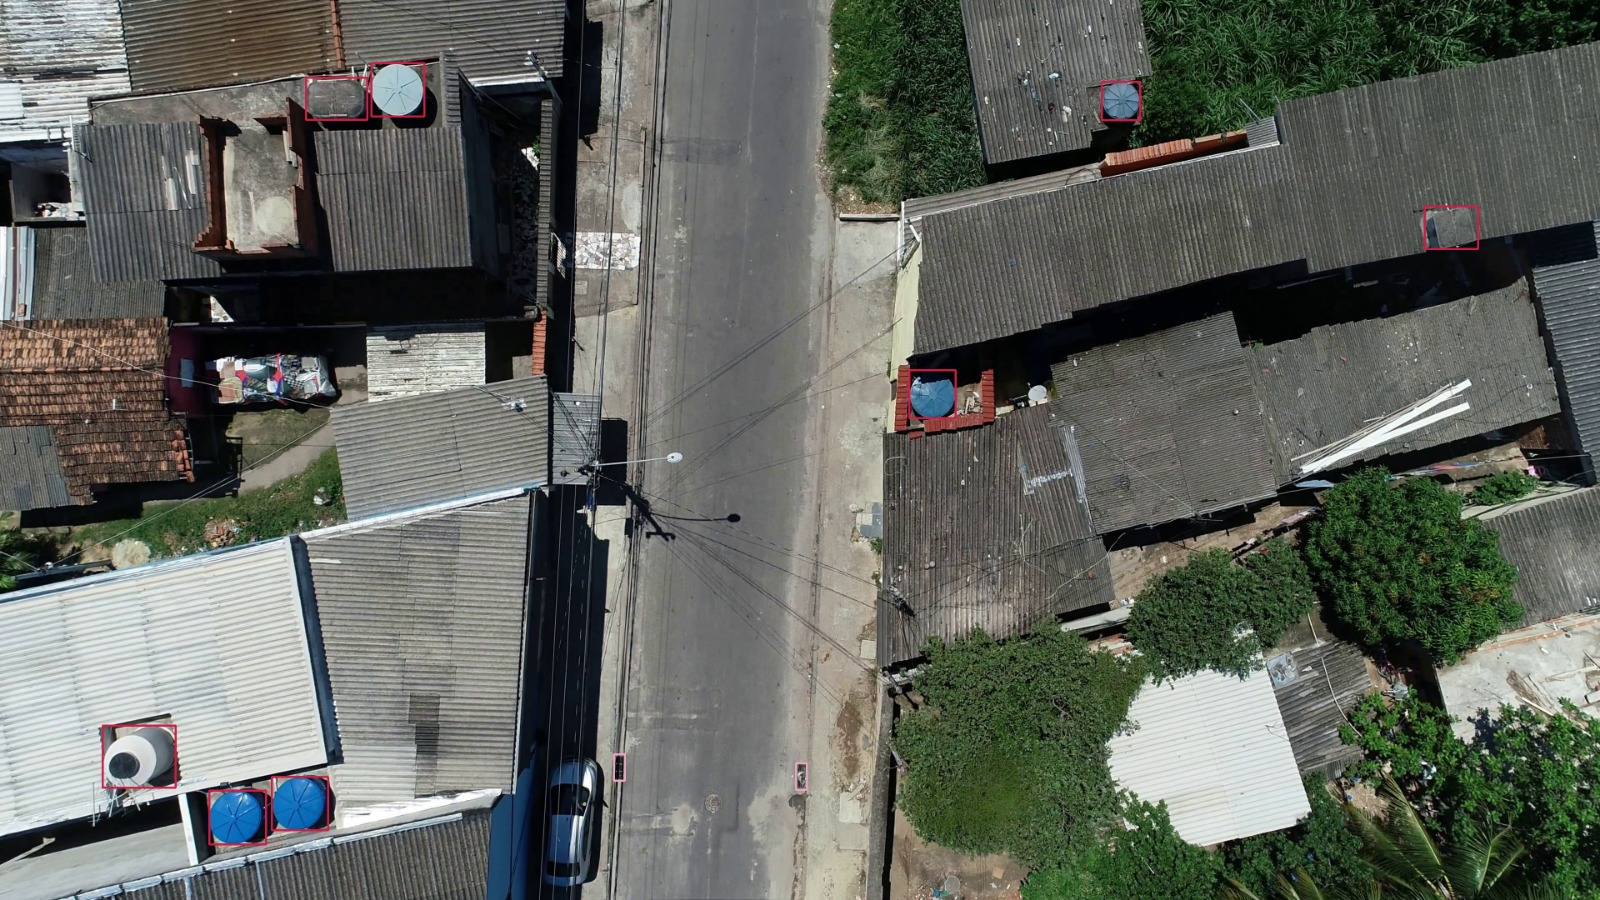
\includegraphics[width=0.9\linewidth]{figures/datasets/mbgv2_annotated_examples.jpeg}
    \caption{Beispielhafte manuell annotierte Drohnenaufnahmen aus dem MBG-V2-Datensatz.
        Markiert sind potenzielle Brutstätten von \textit{Aedes aegypti} wie Wassertanks und
        Straßeneinläufe, die aufgrund ihrer geringen Objektgröße und komplexen urbanen
        Hintergrundstrukturen eine besondere Herausforderung für die automatische
        Objekterkennung darstellen.}
    \label{fig:mbgv2_detection_examples}
\end{figure}

\subsection{Automatische Annotation und Objektverfolgung in Videodaten}

Im Vergleich zu Einzelbildern bieten video-basierte Datensätze den
wesentlichen Vorteil, dass neben räumlichen Informationen auch zeitliche
Zusammenhänge explizit genutzt werden können. Objekte weisen über
aufeinanderfolgende Frames hinweg eine visuelle und räumliche Kontinuität
auf, die gezielt für die Objekterkennung und Objektverfolgung ausgenutzt
werden kann. Aus diesem Grund gewinnen Ansätze, die Objektdetektion und
Objektverfolgung in Videodaten kombinieren, zunehmend an Bedeutung
\cite{bewley2016sort, wojke2017deepsort}.

Ein grundlegendes Prinzip solcher Verfahren besteht darin, zunächst in
jedem Frame Objekte mittels eines Detektionsmodells zu lokalisieren und
diese Detektionen anschließend über die Zeit hinweg konsistenten
Objektidentitäten zuzuordnen. Bekannte Tracking-Algorithmen wie SORT
\cite{bewley2016sort} oder DeepSORT \cite{wojke2017deepsort} nutzen hierzu
Bewegungsmodelle sowie visuelle Merkmalsrepräsentationen, um Objekte auch
bei kurzzeitigen Verdeckungen oder unzuverlässigen Detektionen stabil
verfolgen zu können.

Ein Beispiel für die erfolgreiche Anwendung dieses Ansatzes in einer
verwandten Anwendungsdomäne ist die automatische Detektion und Verfolgung
von Fischen in natürlichen Unterwasserumgebungen. In einer in
\textit{PLOS ONE} veröffentlichten Studie wird ein Verfahren vorgestellt,
das einen YOLO-basierten Objekterkenner mit dem DeepSORT-Tracking-
Algorithmus kombiniert, um Fische in Unterwasservideos zuverlässig zu
detektieren und über lange Videosequenzen hinweg zu verfolgen
\cite{fishtracking2024}.

\begin{figure}[H]
    \centering
    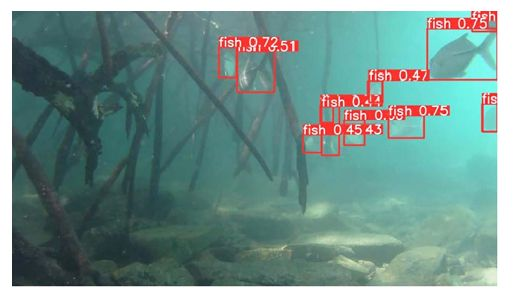
\includegraphics[width=0.9\linewidth]{figures/related_work/fish_tracking_example.jpeg}
    \caption{Beispielhafte Kombination aus YOLO-basierter Objektdetektion
        und DeepSORT-Objektverfolgung in Unterwasservideos. Die Abbildung
        veranschaulicht die zeitlich konsistente Verfolgung detektierter
        Objekte über mehrere Frames hinweg und dient als methodisches
        Beispiel für die Nutzung von Tracking-Informationen zur Reduktion
        manuellen Annotierungsaufwands. Adaptiert nach \cite{fishtracking2024}.}
    \label{fig:yolo_deepsort_fish}
\end{figure}

Darüber hinaus hebt die Literatur hervor, dass Objektverfolgung dazu
beiträgt, framebasierte Detektionsergebnisse zeitlich zu stabilisieren
und Fehlklassifikationen zu reduzieren, indem inkonsistente
Einzelvorhersagen über mehrere Frames hinweg ausgeglichen werden
\cite{wojke2017deepsort}. Diese Eigenschaft ist insbesondere bei
video-basierten Datensätzen mit begrenzter manueller Annotation von
zentraler Bedeutung.

Im Kontext der automatischen Annotation bilden die durch Objektverfolgung
gewonnenen zeitlich konsistenten Objektidentitäten eine wesentliche
Grundlage für semi-supervised Lernverfahren und Pseudo-Labeling-Ansätze.
Aktuelle Arbeiten zeigen, dass bei der video-basierten Objekterkennung
eine begrenzte Anzahl manuell annotierter Frames effektiv durch
automatisch generierte Labels ergänzt werden kann, ohne die
Modellleistung signifikant zu beeinträchtigen \cite{li2022ssvod}. Solche
Ansätze stellen einen vielversprechenden Weg dar, um den manuellen
Annotierungsaufwand in umfangreichen Videodatensätzen signifikant zu
reduzieren und gleichzeitig robuste Detektionsmodelle zu trainieren.


\subsection{Semi-supervised Learning und Pseudo-Labeling}

Tiefenlern-basierte Objekterkennungsmodelle erfordern in der Regel große Mengen manuell
annotierter Trainingsdaten. Insbesondere bei video-basierten Datensätzen ist eine vollständige manuelle Annotation aller Frames aufgrund des hohen zeitlichen und personellen Aufwands nur eingeschränkt praktikabel. Aus diesem Grund gewinnen semi-supervised Lernverfahren, die mit einer begrenzten Menge annotierter Daten arbeiten, zunehmend an Bedeutung \cite{zhu2005ssl}.

Ein weit verbreiteter Ansatz im semi-supervised Learning ist das sogenannte Pseudo-Labeling. Dabei wird ein zunächst mit annotierten Daten trainiertes Modell verwendet, um Vorhersagen auf unannotierten Daten zu erzeugen, welche anschließend als zusätzliche Trainingslabels genutzt werden \cite{lee2013pseudo}. Ziel dieses Verfahrens ist es, den manuellen Annotierungsaufwand zu reduzieren und gleichzeitig die Lernbasis des Modells zu erweitern.

\begin{figure}[H]
    \centering
    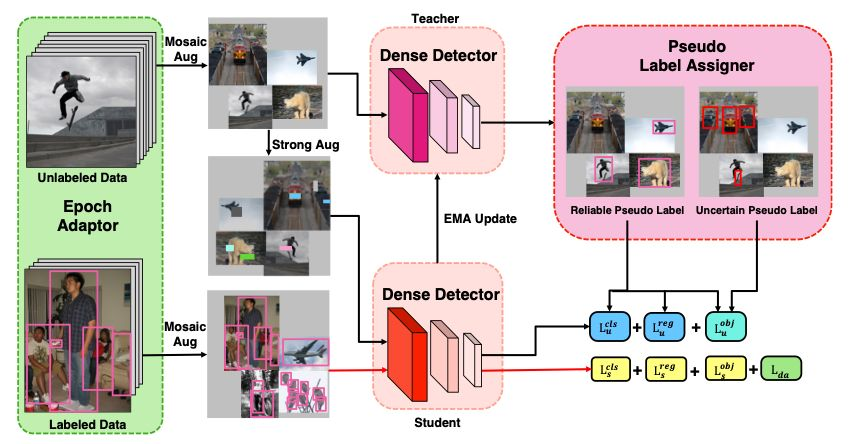
\includegraphics[width=0.95\linewidth]{figures/related_work/efficient_teacher_pipeline.jpeg}
    \caption{Schematische Darstellung eines Pseudo-Labeling-basierten
        semi-supervised Lernverfahrens für die Objekterkennung nach dem
        Teacher-Student-Prinzip. Ein mit annotierten Daten trainiertes
        Modell (Teacher) erzeugt Pseudo-Labels für unannotierte Daten,
        welche nach einer Konfidenzfilterung für das erneute Training eines
        Student-Modells genutzt werden. Die Abbildung dient der
        konzeptionellen Veranschaulichung und ist adaptiert nach
        \cite{liu2021efficient}.}
    \label{fig:efficient_teacher_pipeline}
\end{figure}


In den letzten Jahren wurden zahlreiche Pseudo-Labeling-basierte Methoden speziell für die Objekterkennung entwickelt. Ansätze wie Efficient Teacher nutzen ein Teacher-Student-Paradigma, um robuste Pseudo-Labels aus unannotierten Daten zu generieren und dadurch die Leistung bei begrenzter Annotation zu verbessern \cite{liu2021efficient}. Solche Methoden zeigen, dass semi-supervised Lernverfahren insbesondere in datenarmen Szenarien eine leistungsfähige Alternative zu vollständig überwachten Ansätzen darstellen können.

Für video-basierte Objekterkennungsprobleme bietet semi-supervised Learning zusätzliche
Vorteile, da zeitliche Zusammenhänge zwischen aufeinanderfolgenden Frames berücksichtigt werden können. Arbeiten wie SSVOD demonstrieren, dass eine kleine Anzahl manuell annotierter Frames ausreicht, um mithilfe von Pseudo-Labeling und zeitlichem Kontext Informationen aus den verbleibenden, unannotierten Frames effektiv zu nutzen \cite{li2022ssvod}. Diese Ansätze stellen einen vielversprechenden Weg dar, um den manuellen Annotierungsaufwand bei umfangreichen Videodatensätzen signifikant zu reduzieren.

Vor diesem Hintergrund bilden semi-supervised Learning und Pseudo-Labeling zentrale Konzepte für die Entwicklung automatischer Annotationsverfahren in video-basierten Szenarien.

\subsection{Einordnung der vorliegenden Arbeit}

Die in den vorherigen Abschnitten vorgestellten Arbeiten zeigen, dass die Detektion von
Mückenbrutstätten mithilfe von Luft- und Drohnenbildern ein aktives und relevantes
Forschungsgebiet darstellt. Bestehende Ansätze basieren dabei überwiegend auf vollständig
überwachten Lernverfahren, bei denen alle Trainingsdaten manuell annotiert werden müssen
\cite{passos2023augmented, knoblauch2023breeding}. Insbesondere bei video-basierten
Datensätzen führt dieser Ansatz zu einem hohen zeitlichen und personellen Aufwand, der
die Skalierbarkeit solcher Verfahren erheblich einschränkt.

Arbeiten aus verwandten Anwendungsdomänen zeigen, dass die Kombination aus
Objekterkennung, Objektverfolgung und automatischer Annotation ein vielversprechender
Ansatz zur Reduktion des manuellen Annotierungsaufwands ist. Dies konnte sowohl in
biologischen Anwendungsfällen, wie der Detektion und Verfolgung von Fischen in Videodaten,
als auch in allgemeinen video-basierten Objekterkennungsproblemen gezeigt werden
\cite{fishtracking2024, wojke2017deepsort}.

Darüber hinaus belegen aktuelle Studien im Bereich des semi-supervised Learning, dass
Pseudo-Labeling-basierte Verfahren in der Lage sind, mit einer begrenzten Anzahl manuell
annotierter Daten robuste Modelle zu trainieren \cite{lee2013pseudo, li2022ssvod}.
Insbesondere bei Videodaten bietet die Nutzung zeitlicher Konsistenz zusätzliche
Möglichkeiten, um automatisch generierte Labels zu stabilisieren und deren Qualität zu
verbessern.

Die vorliegende Arbeit knüpft an diese Erkenntnisse an und kombiniert erstmals die
video-basierte Detektion von Mückenbrutstätten mit einem iterativen, semi-supervised
Ansatz zur automatischen Annotation. Durch die gezielte Auswahl weniger manuell
annotierter Frames, die Nutzung von Objektverfolgung zur Sicherstellung zeitlicher
Konsistenz sowie die iterative Erweiterung des Trainingsdatensatzes mittels
Pseudo-Labeling wird ein skalierbarer Ansatz zur Annotation umfangreicher Videodaten
vorgestellt. Damit positioniert sich diese Arbeit an der Schnittstelle zwischen
vollüberwachter Objekterkennung und automatischer, datengetriebener Annotation in
video-basierten Szenarien.

\begin{figure}[H]
    \centering
    \begin{tikzpicture}[
            box/.style={draw, rounded corners, minimum width=4cm, minimum height=1cm, align=center},
            arrow/.style={->, thick}
        ]
        \node[box] (sup) {Fully supervised\\Object Detection\\(manuelle Annotation)};
        \node[box, below=1.2cm of sup] (this) {Diese Arbeit\\Detection + Tracking\\Semi-supervised Annotation};
        \node[box, below=1.2cm of this] (unsup) {Fully automatic\\Ansätze};

        \draw[arrow] (sup) -- (this);
        \draw[arrow] (this) -- (unsup);
    \end{tikzpicture}
    \caption{Einordnung der vorliegenden Arbeit zwischen vollständig überwachten und
        automatischen Ansätzen zur Objekterkennung in Videodaten.}
    \label{fig:work_positioning}
\end{figure}
